% !TEX root = ../notes_template.tex
\chapter{Prokaryotic Transcriptomes}\label{chp:prokaryotic_transcriptomes}

\minitoc

\section{Introduction}

Our perception of a bacterial transcriptome once used to be simple: mRNA, tRNA or rRNA genes are neatly arranged along the 
chromosome and expressed as distinct mono-cistronic or polycistronic transcripts. However, over the last two decades, 
new global methods have reported dense transcript patterns across the bacterial chromosome, and discovered a plethora of 
small regulatory RNAs (sRNAs) and antisense transcripts \cite{Sharma2014}. 

Prokaryotic mRNA are synthesized in the cytoplasm and do not require transport from the nucleus (Clark and Pazdernik, 2013). 
They also do not require processing and can begin translation immediately after the transcription is complete. Most mRNA 
contain a sequence at the 5' end of the mRNA prior to the AUG start codon, termed 5' untranslated region (5' UTR) 
(Meijer and Thomas, 2002) and a region following the stop codon, the 3' UTR. Most prokaryotic mRNA contain a sequence in 
the 5' UTR to position ribosomes for translation. This sequence is named after its discoverers as the Shine-Dalgarno sequence \cite{Goss2016}. 

The Shine-Dalgarno sequence is present in nearly all prokaryotic mRNA; however, recent evidence has shown that there are 
prokaryotic mRNAs that lack a Shine-Dalgarno sequence in the 5' UTR (Londei, 2005) or lack a 5' UTR completely. These mRNAs 
appear to be more common in primitive prokaryotes, such as archaea, in which initiation of translation on leaderless transcripts 
is thought to be the evolutionary oldest mechanism. The mechanism of how these prokaryotes distinguish the start codon is not known \cite{Goss2016}. 

In prokaryotic cells, a single mRNA may code for several proteins. Each message on the mRNA is contained in a single 'open reading frame' 
a sequence of codons bound by start and stop codons. There are no start or stop codons within the reading frame itself. 
The arrangement of messages in tandem along a single strand of mRNA allows the proteins (often called gene products) to 
be translated simultaneously; these gene products are often related in function. Because mRNAs are single stranded, some 
mRNA molecules are able to base-pair within themselves and can form secondary and tertiary three-dimensional structures. 
These structures can regulate the synthesis of polypeptides in the polycistronic mRNA. One example of this mechanism is 
MS2 bacteriophage (Kozak, 1983). The A protein is coded at the 5' end of the polycistronic message, but is needed in only 
small quantities. The 5' end of the mRNA is often blocked by tertiary folding of the mRNA allowing only limited translation 
of the A protein while allowing translation to occur at more accessible sites downstream from the A gene.

\begin{figure}[!ht]
    \centering
    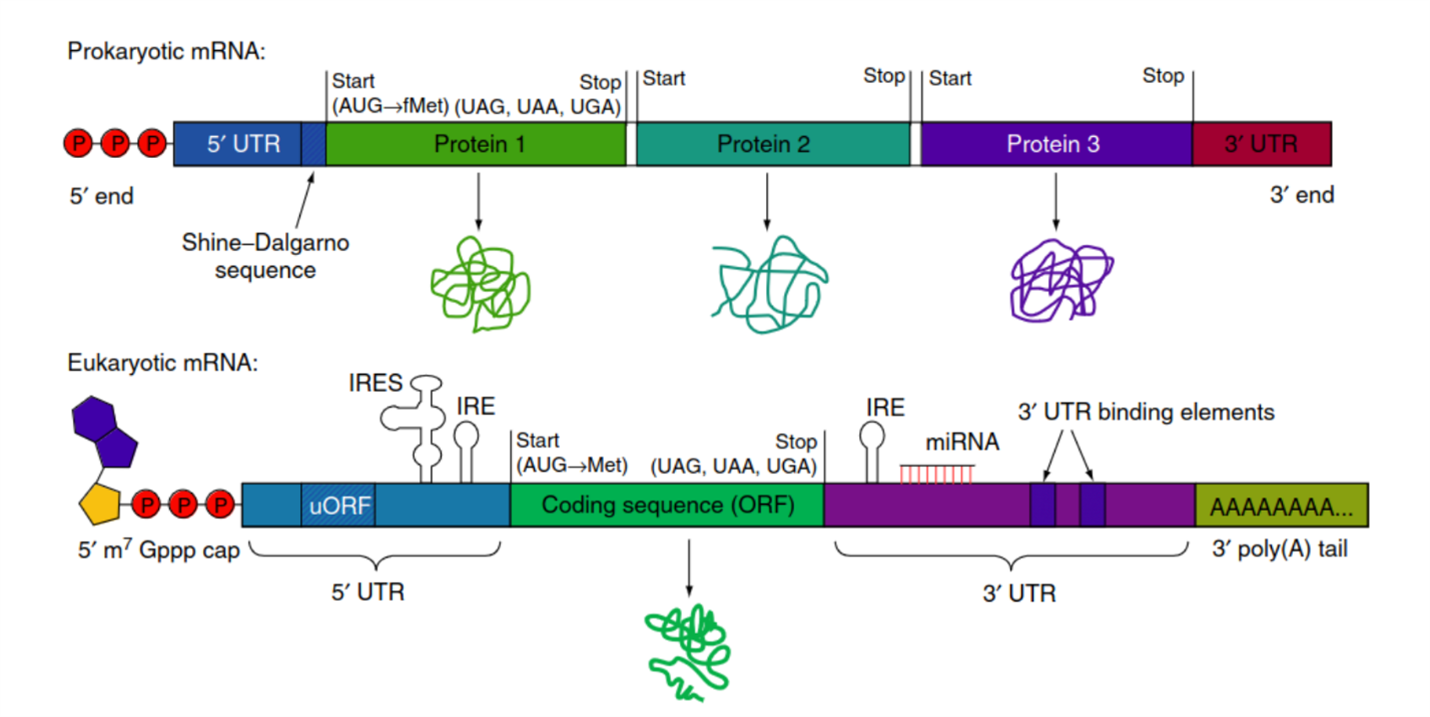
\includegraphics[width=1\linewidth]{./figure/mrna_comparison.png}
    \caption{Schematic diagram of prokaryotic (top) and eukaryotic (bottom) mRNA. Bars indicate the relative length of the regions. 
    Borrowed from \citetitle{Goss2016} \cite{Goss2016}.}
    \label{fig:mrna_comparison}
\end{figure}

\section{Prokaryotic vs Eukaryotic mRNA}
\subsection{Common structures}
The structures of both eukaryotic and prokaryotic genes involve several nested sequence elements. Each element has a specific 
function in the multi-step process of gene expression. The sequences and lengths of these elements vary, but the same general 
functions are present in most genes. Although DNA is a double-stranded molecule, typically only one of the strands encodes 
information that the RNA polymerase reads to produce protein-coding mRNA or non-coding RNA. This 'sense' or 'coding' strand, 
runs in the 5' to 3' direction where the numbers refer to the carbon atoms of the backbone's ribose sugar. The open reading frame (ORF) 
of a gene is therefore usually represented as an arrow indicating the direction in which the sense strand is read.  

Regulatory sequences are located at the extremities of genes. These sequence regions can be next to the transcribed region 
(the promoter) or separated by many kilobases (enhancers and silencers). The promoter is located at the 5' end of the gene 
and is composed of a core promoter sequence and a proximal promoter sequence. The core promoter marks the start site for 
transcription by binding RNA polymerase and other proteins necessary for copying DNA to RNA. The proximal promoter region 
binds transcription factors that modify the affinity of the core promoter for RNA polymerase. Genes may be regulated by 
multiple enhancer and silencer sequences that further modify the activity of promoters by binding activator or repressor 
proteins. Enhancers and silencers may be distantly located from the gene, many thousands of base pairs away. The binding 
of different transcription factors, therefore, regulates the rate of transcription initiation at different times and in 
different cells.  

Regulatory elements can overlap one another, with a section of DNA able to interact with many competing activators and repressors 
as well as RNA polymerase. For example, some repressor proteins can bind to the core promoter to prevent polymerase binding. For 
genes with multiple regulatory sequences, the rate of transcription is the product of all of the elements combined. Binding of 
activators and repressors to multiple regulatory sequences has a cooperative effect on transcription initiation.  

Although all organisms use both transcriptional activators and repressors, eukaryotic genes are said to be 'default off', 
whereas prokaryotic genes are 'default on'. The core promoter of eukaryotic genes typically requires additional activation 
by promoter elements for expression to occur. The core promoter of prokaryotic genes, conversely, is sufficient for strong 
expression and is regulated by repressors.  

An additional layer of regulation occurs for protein coding genes after the mRNA has been processed to prepare it for 
translation to protein. Only the region between the start and stop codons encodes the final protein product. The flanking 
untranslated regions (UTRs) contain further regulatory sequences. The 3' UTR contains a terminator sequence, which marks 
the endpoint for transcription and releases the RNA polymerase. The 5' UTR binds the ribosome, which translates the 
protein-coding region into a string of amino acids that fold to form the final protein product. In the case of genes for 
non-coding RNAs the RNA is not translated but instead folds to be directly functional.

\subsection{Eukaryotes}
The structure of eukaryotic genes includes features not found in prokaryotes. Most of these relate to post-transcriptional 
modification of pre-mRNAs to produce mature mRNA ready for translation into protein. Eukaryotic genes typically have more 
regulatory elements to control gene expression compared to prokaryotes. This is particularly true in multicellular eukaryotes, 
including humans, where gene expression varies widely among different tissues.  

A key feature of the structure of eukaryotic genes is that their transcripts are typically subdivided into exon and intron 
regions. Exon regions are retained in the final mature mRNA molecule, whereas intron regions are excised during post-transcriptional 
processing. Indeed, the intron regions of a gene can be considerably longer than the exon regions. Once spliced together, 
the exons form a single continuous protein-coding region, and the splice boundaries are not detectable. Eukaryotic 
post-transcriptional processing also adds a 5' cap to the start of the mRNA and a poly-adenosine tail to the end of the mRNA. 
These additions stabilise the mRNA and direct its transport from the nucleus to the cytoplasm, although neither of these 
features are directly encoded in the structure of a gene.

\begin{figure}[!ht]
    \centering
    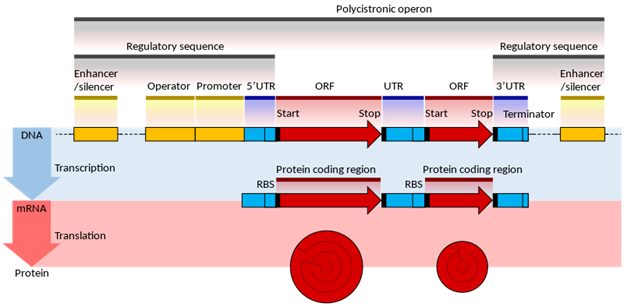
\includegraphics[width=1\linewidth]{./figure/eukaryote_mrna.png}
    \caption{The structure of a eukaryotic protein-coding gene. Regulatory sequence controls when and where expression occurs 
    for the protein coding region (red). Promoter and enhancer regions (yellow) regulate the transcription of the gene into a 
    pre-mRNA which is modified to remove introns (light grey) and add a 5' cap and poly-A tail (dark grey). The mRNA 5' and 3' 
    untranslated regions (blue) regulate translation into the final protein product. Borrowed from \citetitle{Schafee2017} \cite{Schafee2017}.}
    \label{fig:eukaryote_mrna}
\end{figure}

\subsection{Prokaryotes}
The overall organisation of prokaryotic genes is markedly different from that of the eukaryotes. The most obvious difference 
is that prokaryotic ORFs are often grouped into a polycistronic operon under the control of a shared set of regulatory sequences. 
These ORFs are all transcribed onto the same mRNA and so are co-regulated and often serve related functions. Each ORF typically 
has its own ribosome binding site (RBS) so that ribosomes simultaneously translate ORFs on the same mRNA. Some operons 
also display translational coupling, where the translation rates of multiple ORFs within an operon are linked. This can 
occur when the ribosome remains attached at the end of an ORF and simply translocates along to the next without the need 
for a new RBS. Translational coupling is also observed when translation of an ORF affects the accessibility of the next 
RBS through changes in RNA secondary structure. Having multiple ORFs on a single mRNA is only possible in prokaryotes because 
their transcription and translation take place at the same time and in the same subcellular location \cite{Schafee2017}.  

The operator sequence next to the promoter is the main regulatory element in prokaryotes. Repressor proteins bound to the 
operator sequence physically obstruct the RNA polymerase enzyme, preventing transcription. Riboswitches are other important 
regulatory sequences commonly present in prokaryotic UTRs. These sequences switch between alternative secondary structures 
in the RNA depending on the concentrations of key metabolites. The secondary structures then either block or reveal important 
sequence regions such as RBSs. Introns are extremely rare in prokaryotes and therefore do not play a significant role in 
prokaryotic gene regulation \cite{Schafee2017}.

\begin{figure}[!ht]
    \centering
    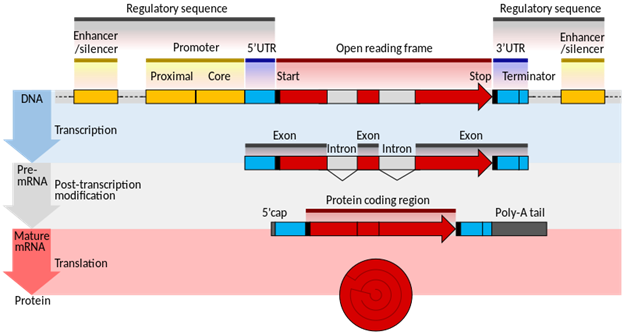
\includegraphics[width=1\linewidth]{./figure/prokaryote_mrna.png}
    \caption{The structure of a prokaryotic operon of protein-coding genes. Regulatory sequence controls when expression 
    occurs for the multiple protein coding regions (red). Promoter, operator and enhancer regions (yellow) regulate the 
    transcription of the gene into an mRNA. The mRNA untranslated regions (blue) regulate translation into the final protein 
    products. Borrowed from \citetitle{Schafee2017} \cite{Schafee2017}.}
    \label{fig:prokaryote_mrna}
\end{figure}

\begin{figure}[!ht]
    \centering
    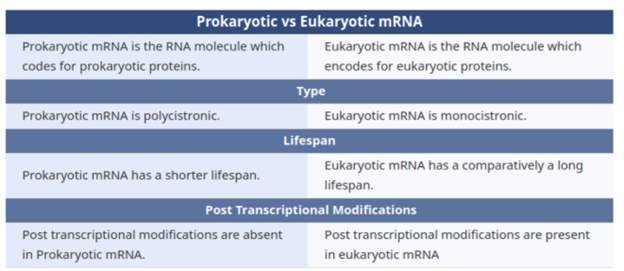
\includegraphics[width=1\linewidth]{./figure/mrna_comparison_table.png}
    \caption{Table comparison. Borrowed from somewhereelse.}
    \label{fig:mrna_comparison_table}
\end{figure}

\section{RNA-seq}
While a major challenge for early bacterial RNA-seq experiments was the presence of highly abundant RNA species like rRNAs 
and tRNAs, which make up more than 95\% of the RNA pool in a bacterial cell, this issue was overcome in eukaryotes by solely 
reverse-transcribing poly(A)-tailed mRNAs via oligo-d(T) priming during cDNA library preparation. Since poly(A)-tails represent 
a degradation signal in bacteria, several strategies for rRNA removal including oligonucleotide-based removal of rRNAs 
with magnetic beads or size fractionation using gel electrophoresis were employed  \cite{Bischler2015}.  

In a typical RNA-seq experiment total RNA or a fraction thereof is first converted into cDNA in a reverse-transcription 
reaction, followed by PCR-based amplification of the library. Different library protocols are available, which are highly 
specific for the applied sequencing technique but can be subdivided into strand-specific and non-strand-specific protocols. 
Non-strand-specific protocols, for example, based on random hexamer priming and ligation of adapters to double-stranded 
cDNA have the drawback that they lose the information whether sequencing reads originate from the sense or the antisense 
strand. To overcome this problem, strand-specific protocols have been developed including direct sequencing of first strand 
cDNA, template switching PCR, RNA C to U conversion using bisulfite or second strand synthesis with dUTP followed by degradation 
after adapter ligation \cite{Bischler2015,Sharma2014}.  

RNA-seq-based mapping of bacterial transcript boundaries enables a global elucidation of operon structures and facilitates 
annotation of untranslated regions (UTRs) of protein coding genes, which potentially contain gene regulatory elements. 
Additionally, it can improve genome annotation by providing extensive information on transcriptional start sites (TSS), 
untranslated regions (UTRs) of mRNA genes, and previously unknown open reading frames (ORFs) or sRNA genes \cite{Sharma2014}. 

\section{Differential RNA-seq}
Differential RNA-seq (dRNA-seq) method allows for global annotation of all expressed transcriptional start sites (TSS) under 
the examined growth condition in an organism of interest in one sequencing experiment. While it was originally developed to 
study the primary transcriptome of the major human pathogen Helicobacter pylori it has since been successfully applied for 
determination of TSS in a wide range of pro- and eukaryotic organisms. With >1900 unique TSS and at least one antisense TSS 
to 50\% of all genes, the dRNA-seq approach revealed a very complex and compact transcriptional output from the small 
\textit{H. pylori} genome and an unexpected number of \(\ge\)60 sRNA  \cite{Schafee2017}.

\begin{figure}[!ht]
    \centering
    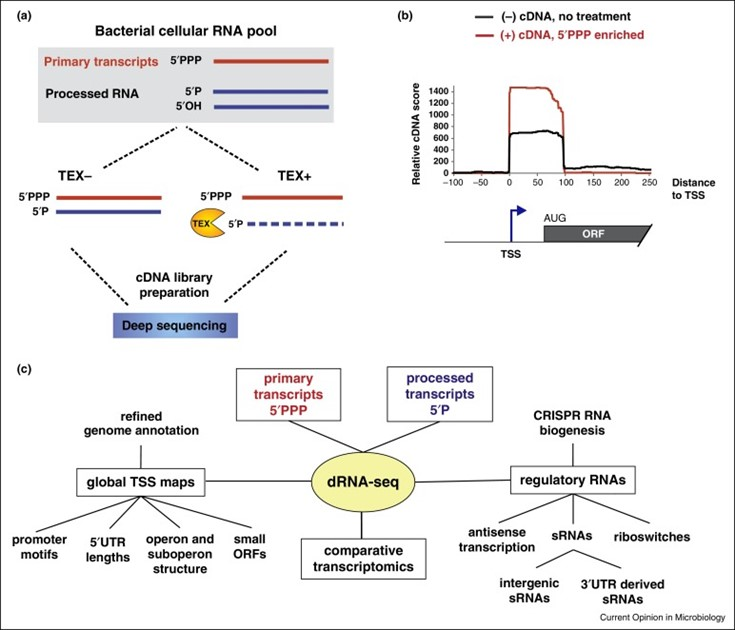
\includegraphics[width=1\linewidth]{./figure/dif_rnaseq.jpg}
    \caption{Rationale and output of the dRNA-seq approach. (a) Enrichment of primary transcripts using 5'-phosphate-dependent 
    terminator exonuclease (TEX). The bacterial RNA pool consists of primary transcripts with a 5'PPP and processed RNAs 
    with a 5'P or 5'OH. RNAs with a 5' OH group are not accessible for 5'-linker ligation during cDNA library constructions 
    and, thus, will not be represented in the cDNA library. For the construction of dRNA-seq libraries, each RNA sample is 
    split into two parts. One half remains untreated (TEX-), whereas the other half is treated with TEX which specifically 
    degrades RNAs with a 5' P, and thereby enriches for primary transcripts with a 5'PPP in relative terms. Upon differential 
    TEX treatment, both samples are converted into a cDNA library and analyzed by deep sequencing. (b) A dRNA-seq specific 
    cDNA enrichment pattern can be observed at the primary 5' ends of genes. Treatment with TEX (red curve; (+) library) 
    redistributes the cDNAs towards the nuclease-protected 5'-end, yielding a sawtooth-like profile with an elevated sharp 
    5' flank which can be used to annotate the TSS (blue arrow) of a gene of interest (grey bar). Note that dRNA-seq reads 
    cluster towards a gene's 5' end if no fragmentation is used. (c) Schematic summary of information that can be gained 
    from dRNA-seq to uncover transcriptome features and refine genome annotation. Borrowed from \citetitle{Sharma2014} \cite{Sharma2014}.}
    \label{fig:diff_rnaseq}
\end{figure}